% 
% \glsresetentrylist

\par 
This thesis focuses on the application of \acrlong{ml} to the characterisation of quantum mechanical systems
    through use of quantum simulators, 
    so it is pertinent first to introduce the vocabulary of \gls{qm}. 
It is impossible, however, to succinctly capture the entire discipline; 
    in this chapter we will only introduce concepts utilised throughout.
For completeness, we elucidate some fundamental topics of linear algebra and quantum theory in \cref{apdx:fundamentals},
    but consider them too cumbersome to include in the main text. 
For a more complete and general introduction to \gls{qm}, the reader is referred to \cite{griffiths2018introduction, susskind2014quantum}.
Likewise, in this chapter we quickly summarise the key aspects of quantum computation, 
    but for further details, we recommend unfamiliar readers to consult \cite{rieffel2011quantum}, 
    while a more complete discussion is presented in \cite{nielsen2002quantum}.

%%%%%%%%%%%%%%%% QUANTUM MECHANICS %%%%%%%%%%%%%%%%%
\section{Quantum mechanics}\label{sec:qm}

At any time, $t$, a quantum system, \gls{q}, can be described by its \emph{wavefunction}, $\Psi(t)$, 
    which contains all information about \gls{q}. 
In analogy with Newton's second law of motion, 
    which allows for the determination of a particle's position at any time, $\vec{r}(t)$, 
    given its conditions -- its initial position, $\vec{r}(t_0)$ and momentum --   
    quantum \emph{equations of motion} can describe the evolution of \gls{q} through its wavefunction \cite{dirac1981principles}. 
One proposal\footnotemark \ for the equation of motion 
    to describe the evolution of the wavefunction under known conditions, 
    i.e. determining $\Psi(t)$ from $\Psi(t_0) \ \forall t > t_0$, 
    is the \emph{\schrodinger equation}  \cite{griffiths2018introduction, mart2020introduce, nelson1966derivation}.
\footnotetext{
    The most noteworthy alternative formalism, due to Heisenberg \cite{heisenberg1985quantentheoretische}, 
    was shown equivalent to the \schrodinger picture described here.
}
\par 

Although the \schrodinger equation is a \emph{postulate} of \gls{qm}, 
    i.e. can act as a starting point for \gls{qm} (see \cref{sec:postulates}), 
    we will sketch a brief, informal derivation to elucidate its meaning
    following \cite{susskind2014quantum}.
We have yet to describe the structure of the wavefunction, which we will do in \cref{sec:quantum_info},
    but here we will represent wavefunctions using \emph{Dirac notation} (\cref{sec:dirac_notation}), 
    and can think of them generically as vectors, i.e. $\Psi(t) \rightarrow \ket{\psi(t)}$. 
Suppose we have two such wavefunctions, $\ket{\phi(t)}, \ket{\psi(t)}$ which are functions of time $t > t_0$.
We start with the assumption that \emph{similarity} is conserved between two wavefunctions,
    if they undergo the same transformation 
    (Susskind's \emph{minus first} law of classical mechanics \cite{susskind2014quantum}),

\begin{equation}
    \label{eqn:conservation_simularity}
    \braket{\phi(t) | \psi(t)} = \braket{\phi(t_0) | \psi(t_0)}.
\end{equation}

Then, assuming some equations of motion capture the dynamics of \gls{q}, 
    there exists some evolution operator, $\hat{U}(t)$, which deterministically maps $\ket{\psi(t_o)}$ to $\ket{\psi(t)}$.
That is, 
\begin{equation}
    \label{eqn:unitary_time_evolution}
    \ket{\psi(t)} = \hat{U}(t) \ket{\psi(t_0)},
\end{equation}
    where we have not yet imposed any restrictions on $\hat{U}$. 
We also have the \emph{dual vector}\footnote{see \cref{sec:linear_algebra}} of \cref{eqn:unitary_time_evolution},
\begin{equation}
    \label{eqn:dual_unitary_evolution}
    \bra{\psi(t)} = \bra{\psi(t_o)}\hat{U}^{\dagger}.
\end{equation} 
Combining \crefrange{eqn:conservation_simularity}{eqn:dual_unitary_evolution}, 

\begin{align}
    \begin{split}
        \braket{\phi(t) | \psi(t)} &= \braket{ \phi(t_0) | \hat{U}^{\dag} \hat{U}| \psi(t_o) }
        \\
        \Rightarrow \braket{ \phi(t_0) | \hat{U}^{\dag}(t) \hat{U}(t) | \psi(t_o) } &= \braket{\phi(t_0) | \psi(t_0)}
        \\
        \Rightarrow \hat{U}^{\dag}(t) \hat{U}(t) &= \ident \ \ \ \ \forall t,
    \end{split}
\end{align}
where the result $\hat{U}^{\dag}(t) \hat{U}(t) = \ident$ is the condition for \emph{unitarity} of $\hat{U}(t)$ (\cref{sec:unitary}), 
    so we can claim the quantum wavefunction evolves unitarily. 
\par 

By construction, we require that after zero time, i.e. $t = t_0$, the wavefunction has not changed:
\begin{equation}
    \begin{split}
        \ket{\psi(t = t_0)} = \hat{U}(t = t_0)\ket{\psi(t_0)} = \ket{\psi(t_0)}
        \\ \Rightarrow \hat{U}(t = t_0) = \ident.
    \end{split}
\end{equation}
Without loss of generality we can set $t_0 = 0$, giving $\hat{U}(0) = \ident$. 
Then, let us consider an infinitesimally small time increment $t_0 + \epsilon$:
    again, take $t_0 = 0$ so $t = \epsilon$,  where $\epsilon \gg \epsilon^2$. 
We can say
\begin{equation}
    \hat{U}(\epsilon) = \ident + \mathcal{O}(\epsilon),
\end{equation}
which merely suggests that the time evolution operator
    at very small time is very close to the identity, with some small displacement proportional to the time,
    which must be an operator to act on the wavefunction (vector).
We suppose the form of the offset, so we can write
\begin{equation}
    \hat{U}(\epsilon) = \ident - \epsilon \left(\frac{i}{\hbar} \ho \right),
\end{equation}
    where the inclusion of the phase $-i$ is arbitrary, 
    and we have named as $\ho$ the operator by which the time evolution differs from the identity,
    scaled by the reduced Planck constant, $\hbar = 1.054 \times 10^{-34}$.
In other words, the operator $\ho$ is, generically, the generator of the evolution/dynamics of \gls{q}:
    any difference between $\ket{\psi(t_0)}$ and $\ket{\psi(t)}$ arises solely due to $\ho$. 
So far there is no restriction\footnotemark \ on $\ho$.
    \footnotetext{
        We do restrict $\ho$ to the same dimension as the Hilbert space in question;
        the concept of Hilbert space will be defined in \cref{sec:quantum_info}, 
        but is not needed in this discussion.
    }
Recalling the unitarity condition, and that $\lim_{\epsilon \rightarrow 0} \mathcal{O}(\epsilon^2) \approx 0$, 
    we have:
\begin{equation}
    \label{eqn:hamiltonian_hermiticity}
    \begin{split}
        \hat{U}^{\dag}(\epsilon) \hat{U}(\epsilon) &= \ident
        \\ 
        \Rightarrow 
        \left( \ident + \frac{i}{\hbar} \epsilon \ho^\dag \right) \left( \ident - \frac{i}{\hbar} \epsilon \ho \right)  &= \ident
        \\
        \Rightarrow
        \ident +  \frac{i}{\hbar} \epsilon (\ho^{\dag} - \ho) + \mathcal{O}(\epsilon^2) &= \ident
        \\
        \Rightarrow
        (\ho^{\dag} - \ho) = 0 
        \\
        \Rightarrow
        \ho^{\dag} = \ho.
    \end{split}
\end{equation}
\cref{eqn:hamiltonian_hermiticity} results in the condition for \emph{Hermiticity}, 
    meaning that $\ho$ is an observable of \gls{q}. 
In fact, this is the \emph{Hamiltonian} of the system, described in the next section. 

\par 
We can also use the infinitesimal evolution to see 
\begin{equation}
    \label{eqn:derivation_schrodinger_eqn}
    \begin{split}
        \ket{\psi(t)} &= \hat{U}(t) \ket{\psi(t_0)}
        \\ \Rightarrow \ket{\psi(\epsilon)} &= \hat{U}(\epsilon) \ket{\psi(t_0)}
        \\ \Rightarrow 
        \ket{\psi(\epsilon)} &= \left(\ident - \epsilon \frac{i}{\hbar} \ho \right) \ket{\psi(t_0)}
        \\ \Rightarrow \ket{\psi(\epsilon)} &= \ket{\psi(t_0)} - \epsilon \frac{i}{\hbar} \ho \ket{\psi(t_0)}
        \\ \Rightarrow \frac{\ket{\psi(\epsilon)} - \ket{\psi(t_0)} }{\epsilon}  &= - \frac{i}{\hbar} \ho \ket{\psi(t_0)}.
    \end{split}
\end{equation}
Taking the limit as $\epsilon \rightarrow 0 $, the left hand side of the final line of \cref{eqn:derivation_schrodinger_eqn} is the definition
    of the derivative of the wavefunction, $\frac{d \ket{\psi(t)}}{dt}$. 
Taken together, we have 
\begin{equation}
    \label{eqn:schrodinger}
    \frac{\partial}{\partial t} \ket{\psi(t)} = \frac{-i}{\hbar} \ho \ket{\psi(t_0)},
\end{equation}
    where $\ket{\psi(t)}$ is the wavefunction at time $t$, 
    $\ket{\psi(t_0)}$ is the wavefunction at $t_0$, such that $t > t_0$, 
    $\hbar$ is the reduced Planck constant and 
    $\ho$ is the \emph{Hamiltonian} of \gls{q}. 
For brevity we generally refer to $t_0 = 0$, and absorb $\hbar$ into $\ho$, which will later manifest in the \gls{hamiltonian} scalar parameters. 
\cref{eqn:schrodinger} is the most general form of \emph{\schrodinger equation}, 
    otherwise known as the \emph{time-dependent} \schrodinger equation; 
    we include it as \Cref{postulate:schrodinger_eqn} when describing the fundamentals of \gls{qm} (\cref{sec:postulates}), 
    since it can be seen as an irreducible equation of motion which is essential to the description of quantum systems. 
\par 

As mentioned, we presented this argument in a nonstandard order:
    we started with \cref{eqn:unitary_time_evolution}, which we can now consider the \emph{solution} to the \schrodinger equation, 
    specifically
\begin{equation}
    \label{eqn:unitary_evolution}
    \begin{split}
        \ket{\psi(t)} &= \hat{U}(t) \ket{\psi(0)}
        \\
        \implies \hat{U}(t) &= e^{-i \ho t}.
    \end{split}
\end{equation}
$\hat{U}(t)$ then describes the unitary evolution of the wavefunction of a 
    quantum system according to its Hamiltonian, $\ho$. 
\par 

\subsection{Hamiltonians}\label{sec:hamiltonians}
In the previous section we introduced the \gls{hamiltonian} of \gls{q} as the generator of its 
    time evolution dynamics;
    \glspl{hamiltonian} are of primary importance in this thesis, so it is worth pausing to consider their physical meaning. 
We saw in \cref{eqn:hamiltonian_hermiticity} that $\ho$ is Hermitian;
    the \gls{hamiltonian} is the observable operator (see \Crefrange{postulate:eigenvalues}{postulate:hermiticity} in \cref{sec:postulates}) 
    associated with the system's total energy, 
    i.e. the permitted energy levels of the system are given by the eigenfunctions of $\ho$. 
\par 

The quantum Hamiltonian, $\ho$, is analogous to the \emph{classical} Hamiltonian, 
    which captures all the interactions of a given classical system which contribute to its time evolution.
Knowing the classical \gls{hamiltonian} and the initial conditions -- position and momentum -- 
    Hamilton's equations of motion allow for the calculation of those quantities for the particle 
    in question an infinitesimal time later \cite{susskind2014classical}.    
Likewise, knowledge of the initial wavefunction, $\ket{\psi(t_0)}$, and the system's quantum Hamiltonian, $\ho$, 
    the quantum equation of motion -- namely the \schrodinger equation, \cref{eqn:schrodinger} -- 
    permits the calculation of the wavefunction at later times.
As such the \gls{hamiltonian} must consist of all processes which influence the evolution of \gls{q};
    we will later break the \gls{hamiltonian} into independent \emph{terms} which each correspond to unique physical interactions
    \gls{q} is subject to, in \cref{sec:models}. 
We can think that each process/interaction \gls{q} undergoes contributes to its total energy,
    giving intuition as to why its eigenvalues are the energy levels. 
\par 
% \footnotetext{
%     Aside: the author shares a hometown with the mathematician for whom it is named, William Rowan Hamilton. 
%     It is hoped that, after another 150 years, the next physicist from Trim, Co. Meath, Ireland might 
%     profitably use knowledge of \glspl{hamiltonian} on a functional quantum computer.} 
% }

\glspl{hamiltonian} describe \emph{closed} quantum systems, 
    i.e. where \emph{all} processes and interactions which influence \gls{q} are accounted for. 
Realistic quantum systems are influenced by a myriad of proximal systems, 
    and it is therefore usually infeasible to analytically account for them all. 
Instead, \emph{open} quantum systems' dynamics can, in some cases, be described by Lindbladian operators, which encompass the \gls{hamiltonian} form. 
The Lindblad master equation is a generalisation of the \schrodinger equation, 
    providing the equation of motion for open quantum systems \cite{breuer2002theory, manzano2020short}.
In this thesis we only consider closed models for quantum systems;
    for meaningful impact of the techniques presented here, it will be necessary to expand them to account for the open system dynamics of realistic experiments.
We do, however, show initial progress towards this endeavour by modelling a physical system through a closed Hamiltonian in \cref{chapter:nv}.
\par 

%%%%%%%%%%%%% QUANTUM INFORMATION %%%%%%%%%%%%%
\section{Quantum information}\label{sec:quantum_info}
The wavefunction for a physical system, \gls{q}, is also known as its \emph{state}, 
    a complete mathematical description of the system \cite{preskill1998lecture}.
States are vectors\footnotemark \ of complex numbers;
    the valid state space for \gls{q} is its \emph{Hilbert space}, $\hilbert$,
    which is a generalisation of Euclidean vector space, 
    i.e. $\ket{\psi} \in \hilbert$. 
\footnotetext{We immediately use Dirac notation to represent the state; it is defined in \cref{sec:dirac_notation}.}
The Hilbert space defines the overlap between any two vectors as the \emph{inner product}, $\braket{\psi | \phi}$ (see \cref{sec:linear_algebra}). 
In general\footnotemark, a state can be seen as a \emph{superposition} across a set of orthonormal states, 
    often represented over the system's eigenstates, $\left\{\ket{v_i}\right\}$:
\footnotetext{We expand on this brief description in \cref{sec:states}.}

\begin{subequations}
    \begin{equation}\label{eqn:state_vector}
        \ket{\psi} = \sum\limits_{i} \alpha_i \ket{v_i}
    \end{equation}
    \begin{equation}\label{vector_norm}
        \textrm{subject to} \ \ \ \sum\limits_{i} |\alpha_i|^2 =1, \ \ \ \alpha_i \in \mathbb{C}. 
    \end{equation}
\end{subequations}

The cornerstone of \gls{qm} is the effect of \emph{measurement} on quantum systems: 
    in general \gls{q} can be seen as occupying a multitude of eigenstates as in \cref{eqn:state_vector};
    observing the system forces $\ket{\psi}$ into definite occupation of a measurement basis state,
    where the \emph{probability} that it is measured in each eigenstate $\ket{v_i}$ is given by $\absval{\alpha_i}^2$, 
    according to Born's rule \cite{born1926quantenmechanik}.
$\alpha_i$ are hence named \emph{probability amplitudes} since they inform the probability of measuring the corresponding eigenstate. 
\par 

For a single particle, when the state, \cref{eqn:state_vector}, has two available eigenstates, 
    e.g. the horizontal ($H$) and vertical ($V$) polarisation of a single photon, 
    we can designate \gls{q} as a two-level computational platform, called a \emph{qubit}\footnotemark, 
    analogous to the workhorse of classical computation, the bit. 
A qubit's state vector can then be written as a sum over the two available eigenstates, 
    where we assign vectors to the eigenstates as 
\begin{equation}
    \begin{split}
        \ket{H} = \ket{v_1} = \icol{1 \\ 0 } =: \ket{0}; \\
        \ket{V} = \ket{v_2} = \icol{0 \\ 1} =: \ket{1}. 
    \end{split}
\end{equation}
\footnotetext{
    Here we describe ideal, \emph{logical} qubits as the foundation of computation. 
    In reality, physical qubits are beset by errors, 
    demanding error correction routines such that multiple particles are needed in order to attain a single logical qubit. 
}
The state of a qubit is then given by 
\begin{equation}
    \label{eqn:qubit_state}
    \ket{\psi} = \alpha_1 \ket{v_1} + \alpha_2 \ket{v_2},
\end{equation}
where $\alpha_i \in \mathbb{C}$ and $\absval{\alpha_1}^2 + \absval{\alpha_2}^2 = 1$. 
\par

In general, a qubit requires two orthogonal state vectors to define a \emph{basis};
    we list a number of the usual special cases:
\begin{subequations}
    \label{eqn:bases}
    \begin{equation}
        \label{eqn:basis_x}
        X\textrm{-basis} = \left\lbrace \begin{split}
        \ket{+} &= \frac{1}{\sqrt{2}} \left( \ket{0} + \ket{1} \right)
        \\
        \ket{-} &= \frac{1}{\sqrt{2}} \left( \ket{0} - \ket{1} \right)
        \end{split}
        \right.
    \end{equation}
    \begin{equation}
        \label{eqn:basis_y}
        \begin{split}
        Y\textrm{-basis} = \left\lbrace 
        \begin{split}
            \ket{i} &= \frac{1}{\sqrt{2}} \left( \ket{0} + i \ket{1} \right)
            \\
            \ket{-i} &= \frac{1}{\sqrt{2}} \left( \ket{0} - i \ket{1} \right)
        \end{split}
        \right.        
        \end{split}
    \end{equation}
    \begin{equation}
        \label{eqn:basis_z}
        Z\textrm{-basis} = \left\lbrace \begin{split}
            &\ket{0}
            \\
            &\ket{1}
            \end{split}
            \right .
    \end{equation}
\end{subequations}

A visual tool for representing qubits is the \emph{Bloch sphere}, 
    which presents orthogonal basis states as parallel unit vectors of opposite direction:
    we show each of the bases of \cref{eqn:bases} in \cref{fig:bases}. 

\begin{figure}
    \begin{center}
        \subfloat{
            % 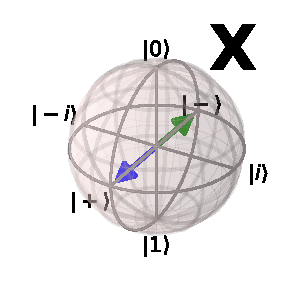
\includegraphics[width=0.3\textwidth]{contextual_review/figures/bloch_x_axis.pdf}
            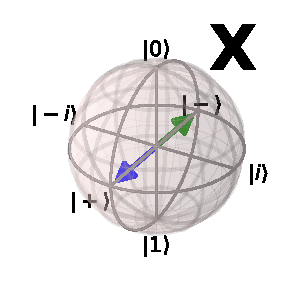
\includegraphics{contextual_review/figures/bloch_x_axis.pdf}
        }
        \qquad
        \subfloat{
            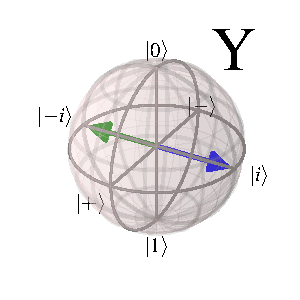
\includegraphics{contextual_review/figures/bloch_y_axis.pdf}
        }
        \qquad
        \subfloat{
            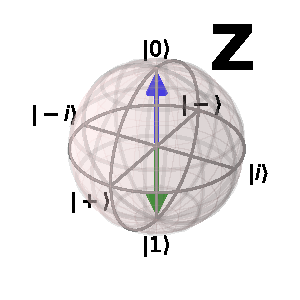
\includegraphics{contextual_review/figures/bloch_z_axis.pdf}
        }
        \qquad
    \end{center}
    \caption[Bloch sphere representation of bases]{
        Bloch sphere representation of bases, where each pair of basis states are shown by blue and green vectors. 
        The $X$-basis has basis vectors $\left\{ \ket{+}, \ket{-}\right\}$; $Y$-basis has $\left\{ \ket{i}, \ket{-i}\right\}$ 
            and $Z$-basis has $\left\{ \ket{0}, \ket{1}\right\}$.
    }
    \label{fig:bases}
\end{figure}

We can make two remarks about basis states for a single qubit:
\begin{easylist}[itemize]
    & Basis states from one basis can be seen as superpositions with respect to alternative bases
    && e.g. in the $X$-basis, $\ket{+}$ is a basis vector, but in the $Z$-basis, $\ket{+} = \frac{\ket{0} + \ket{1}}{\sqrt{2}}$ is a superposition over basis vectors. 
    & Bases are local rotations of each other
    && rotating the $X$-basis through an angle $\nicefrac{\pi}{2}$ about the $Y$-axis results in the $Z$-axis.
\end{easylist}

\par 

As we alluded to in \cref{sec:qm},
    by imposing mathematical structure on quantum systems' states, 
    i.e. representing \gls{q} as a state vector at any time, 
    then operations which alter the state of the system must be matrices, 
    which we will call \emph{operators}. 
In general an $n$-dimensional vector is rotated by an $n \times n$ matrix;
    therefore to rotate the one-qubit state, given by a two-dimensional vector, 
    we require a $2\times2$ operator.
One-qubit operators have the effect of rotating the state vector, 
    which we can again visualise on the Bloch sphere.
By thinking of qubits generically with respect to any basis, we can encode \emph{information} in the qubit's amplitudes,
    by performing operations (or \emph{gates}) upon the qubit, we change the information, 
    i.e. we can design information processing techniques leveraging the infrastructure -- states, operators and measurement -- of \gls{qm}. 
\par 

We introduce a set of special one-qubit operators, the \emph{Pauli matrices},  

\begin{subequations}
    \begin{equation}
        \sx = \begin{pmatrix}
            0 & 1 \\
            1 & 0 
        \end{pmatrix};
    \end{equation}        
    \begin{equation}
        \sy = \begin{pmatrix}
            0 & -i \\
            i & 0 
        \end{pmatrix};
    \end{equation}        
    \begin{equation}
        \sz = \begin{pmatrix}
            1 & 0 \\
            0 & -1
        \end{pmatrix}.
    \end{equation}        
\end{subequations}

The Pauli matrices are used to define rotation operators about 
    their respective axes, and hence are very useful:
    we can break \emph{any} rotation of a qubit into rotations of various angles, $\theta$, about the three axes of the Bloch sphere.
Any single qubit operation can therefore be expressed as a product of
    the \emph{rotation operators}, $\hat{R}_x, \hat{R}_y, \hat{R}_z$, exemplified in \cref{fig:bloch_rotations} and defined for $w \in \{ x,y,z\}$ as
\begin{equation}
    \label{eqn:rotation_operator}
    \begin{split}
        \hat{R}_w\left(\theta\right) &= e^{-i \frac{\theta}{2} \hat{\sigma}_w} 
        = \cos\left(\nicefrac{\theta}{2}\right) \ident - i \sin \left(\nicefrac{\theta}{2}\right) \hat{\sigma}_w.
    \end{split}
\end{equation}
    
\par
The Pauli matrices are observable; 
    in particular, the eigenstates of $\sz$ are the $Z$-basis states:
    $\sz \ket{0} = \ket{0}; \sz \ket{1} = - \ket{1}$.
Recalling the earlier claim that the two-level quantum system (e.g. $H$ and $V$ polarisation of a photon)
    can be mapped to eigenstates of an obserable operator to form a qubit, 
    we term the $Z$-basis the \emph{computational} basis.
By defining the computational basis, we ground abstract computational reasoning in the physical realisation:
    anywhere throughout this thesis where the basis states $\{\ket{0}, \ket{1}\}$ are referenced, 
    we mean the eigenstates of the physical axis which is defined as the $Z$-axis for the system in question. 
% \footnotetext{
%     The terms \emph{eigenstate}, \emph{eigenfunction} and \emph{eigenstate} are interchangeable.
% }
In the computational basis, then, a qubit can be specified as
\begin{equation}
    \label{eqn:computational_qubit}
    \ket{\psi} = \alpha_0 \ket{0} + \alpha_1 \ket{1}.
\end{equation}

\begin{figure}
    \begin{center}
        \subfloat{
            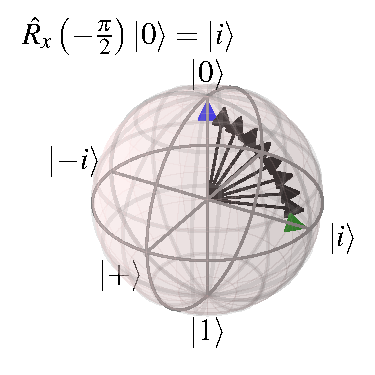
\includegraphics{contextual_review/figures/bloch_rotate_x.pdf}
        }
        \qquad
        \subfloat{
            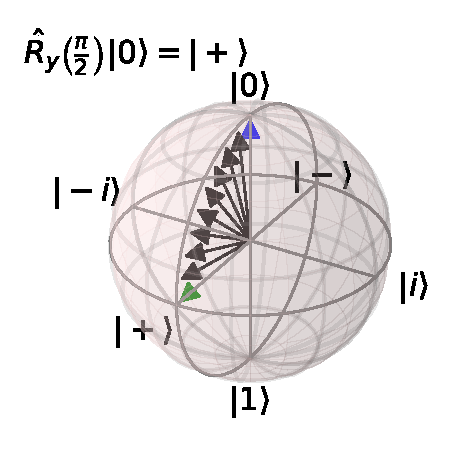
\includegraphics{contextual_review/figures/bloch_rotate_y.pdf}
        }
    \end{center}
    \caption[Rotations on Bloch sphere]{
        Rotations on Bloch sphere. 
        The initial and final states are shown in blue and green respectively, while intermediate states are shown in black. 
        \textbf{Left}, The $Z$-basis unit vector, $\ket{0}$, is rotated about the $X$-axis, resulting in the unit vector along the $Y$-axis. 
        \textbf{Right}, The $Z$-basis unit vector, $\ket{0}$, is rotated about the $Y$-axis, resulting in the unit vector along the $X$-axis. 
    }
    \label{fig:bloch_rotations}
\end{figure}
\par 

The concepts of qubits representing quantum systems, as well as operators
    altering their states and measurement collapsing those states,
    extend straightforwardly to multipartite systems by merging Hilbert spaces through tensor products, 
    as we show in \cref{sec:multipartite}.
% The cases where this is a simple mathematical exercise represent \emph{pure} states;
%     of course this leads to the more intricate topic of \emph{mixed} states and entanglement, 
%     briefly described in \cref{sec:entanglement}.
% In this thesis, however, we are concerned only with pure states, i.e. separable qubits.
While single qubit states are spanned by the Pauli operators, multi-qubit states are spanned by the Pauli group, $\mathbb{G}$: 
    $n$-qubit states are spanned by $\mathbb{G}_n = \left(\mathbb{C}^2\right)^{\otimes n}$.
Multipartite systems can exhibit the strictly non-classical phenomenon of \emph{entanglement}, 
    where the constituent particles can not be described independently, 
    which we briefly detail in \cref{sec:entanglement}. 

\subsection{Expectation values}\label{sec:expectation_value}
\begin{figure}
    \begin{center}
        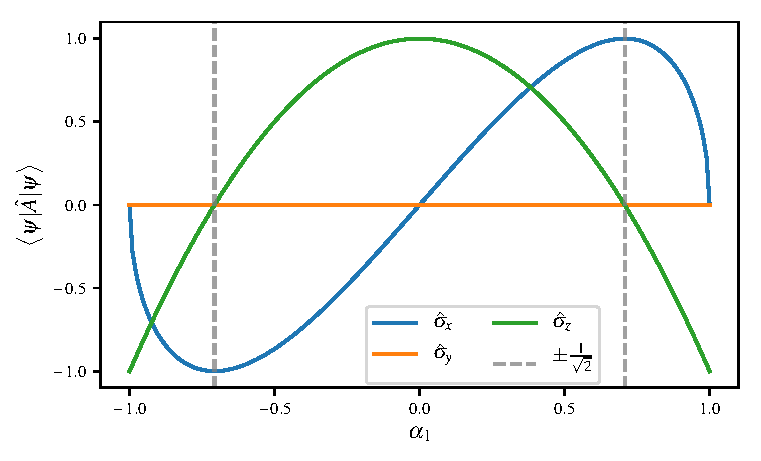
\includegraphics{contextual_review/figures/expectation_values.pdf}
    \end{center}
    \caption[Expectation values]{
        Expectation values of the observable $\hat{A} \in \{ \sx, \sy, \sz\}$ 
            for $\ket{\psi} = \alpha_0 \ket{0} + \alpha_1 \ket{1}$.
            Coefficients are real, varying $\alpha_1 \in \left( -1, 1\right)$, such that $\alpha_0 = \sqrt{1 - \alpha_1^2}$. 
    }
    \label{fig:expectation_values}
\end{figure}

Upon measurement, the state vector of \gls{q} has amplitude associated with only one eigenstate. 
On average, however, the eigenstate to which it would collapse encodes statistical insight on the 
    state prior to measurement. 
In other words, if we prepared $\ket{\psi}$ and measured it -- via some observable, $\hat{A}$ -- 
    and repeat the procedure $N$ times, 
    then as $N \rightarrow \infty$, the average outcome is the \emph{\gls{expectation value}}
    for the system.
\begin{equation}
    \label{eqn:expectation_value}
    \braket{\hat{A}} = \braket{\psi | \hat{A} | \psi} = \sum\limits_{i} \alpha_i \braket{v_i | \hat{A} | v_i},  
\end{equation}
    where $\braket{\hat{A}}$ is the \gls{expectation value} (average) for the observable $\hat{A}$; 
    $\ket{v_i}$ are the eigenstates of $\hat{A}$, and $\alpha_i \in \mathbb{C}$ are the probability amplitudes
    associated with each $\ket{v_i}$ when the state $\ket{\psi}$ is represented as in \cref{eqn:state_vector}.
We show some examples of \glspl{expectation value} for the observable Pauli matrices in \cref{fig:expectation_values}. 
\par 

An underlying theme of this thesis is to flip the usual logic: 
    instead of using knowledge of the system to derive the \gls{expectation value}, per \cref{eqn:expectation_value},
    we will \emph{estimate} \glspl{expectation value}, either through experiment or simulation, 
    and use them to infer the structure of the observable.
This trick enables machine learning routines to reverse engineer 
    the processes \gls{q} is subject to, as we will describe in \cref{part:algorithms}. 

%%%%%%%%%%%%%%% QUANTUM COMPUTING %%%%%%%%%%%%%%%%%%

\section{Quantum simulation and computation}\label{sec:quantum_computation}

Relying on the premise and language of quantum information processing 
    -- states, qubits, operators, measurements and expectation values -- 
    the growing field of \emph{quantum technology} aims to exploit the 
    non-classical statistics yielded by quantum systems in order to retrieve 
    outcomes beyond the capability of their classical counterparts \cite{dowling2003quantum}. 
Applications range from enhanced sensing and metrology \cite{giovannetti2004quantum, giovannetti2011advances}, 
    to highly-secure communication and cryptography protocols \cite{bennett2020quantum, ekert1991quantum, gisin2002quantum}.
The initial motivation for the development of quantum technologies, however, 
    was the  observation that simulating nature at a quantum level would require 
    exponential resources on a classical device, and is therefore only feasible given controllable quantum systems,
    which can accurately emulate their true dynamics \cite{feynman1982simulating, manin1980vychislimoe, benioff1980computer, benioff1982quantum}. 

\par 
The notion of controlling quantum systems to mimic the dynamics of natural quantum systems is tantamount to 
    \emph{quantum simulation} \cite{lloyd1996universal, cirac2012goals}. 
In particular, simulating quantum systems is believed to be of interest for quantum chemistry \cite{cao2019quantum, lanyon2010towards, mcardle2020quantum}, 
    for example leading to advances in the simulation of molecular dynamics \cite{aspuru2005simulated, sparrow2018simulating}.
More generally, however, this led to research into a wider domain of calculations called \emph{quantum computation}
    which considers the information processing capability of controllable quantum systems beyond merely simulating quantum systems. 
Then, \emph{universal \acrlongpl{qc}} (or, \emph{quantum Turing machines}), 
    assume access to \emph{logical} qubits and operations (or \emph{gates}) for the implementation of quantum circuits \cite{deutsch1985quantum}. 
This ignited interest in \emph{quantum algorithms}, which aim to provide some provable advantage 
    \cite{grover1997quantum, simon1997power, bennett1997strengths, bernstein1997quantum, shor1999polynomial}.
Indeed, it was found that the space of problems addressible by such devices
    goes beyond the classical counterpart,
    suggesting there exists a class of quatum algorithms which can offer significant advantage over 
    any feasible algorithm on classical hardware \cite{watrous2008quantum}. 
\par 

Of course, while the advances in algorithmic quantum computation promise huge impact, 
    they are tempered by contemporary experimental constraints, 
    which must deal with the reality that construction and control of 
    quantum devices is a significant challenge.
In constructing \glspl{qc} and dealing with their output, 
    we must account for physical effects which lead to errors, 
    requiring expensive error mitigation schemes in order to be reliable \cite{shor1996fault, aharonov2008fault}.
Furthermore, there are a number of criteria a \gls{qc} must meet before it can be deemed reliable \cite{divincenzo2000physical}. 
\par 

Any two-level quantum system can be used as a qubit, so a range of platforms have emerged in
    attempts to fulfil the potential of quantum computation \cite{humble2019quantum};
    here we provide an incomplete list of quantum architectures together with their primary advantages and limitations.

\begin{description}
    \item[Photonic qubits] (linear optical \glspl{qc}) \cite{kok2007linear}.
    \begin{easylist}
        && existing infrastructure for commercial production of photonics-based technologies suggests the relatively straightforward fabrication 
        of integrated photonic devices at the scale of millions of degrees of freedom \cite{adcock2020advances};
        && photons do not decohere so are useful for encoding information \cite{kovac2002detection};
        && photons do not interfere \cite{dirac1981principles, gerry2005introductory}, 
            making multi-qubit gates difficult to achieve, 
            so information processing must be mediated by non-trivial measurement schemes \cite{raussendorf2003measurement};
        && they are liable to a unique error mechanism -- photon loss -- 
            necessitating novel quantum error correcting codes \cite{vigliar2020error};
        && on-demand single photon generation has not yet been demonstrated,
            although there is significant progress in the area of photon generation \cite{paesani2020near};
        && alternative resource generation is possible through multiplexing, i.e. combining numerous probabilistic photon sources, 
            but this imposes stringent hardware requirements \cite{kaneda2019high}.
        \end{easylist}

    \item[Superconducting qubits] \cite{devoret2004superconducting, kjaergaard2020superconducting}
    \begin{easylist}
        && relatively straightforward to control and couple with each other, enabling high-fidelity two-qubit gates,
        e.g. $99.7 \%$ reached in \cite{kjaergaard2020quantum};
    && difficult to engineer substantial coherence times, although there has been significant recent progress 
        \cite{martinis2014ucsb, wendin2017quantum},
        e.g. $T_1 \approx \mathcal{O}(\textrm{ms})$ in \cite{pop2014coherent};
    && require cryogenic temperatures for operation, demanding expensive and cumbersome infrastructure \cite{devoret2004superconducting};
    && arbitrary qubit connectivity at scale is yet to be demonstrated \cite{kjaergaard2020superconducting};
    && methods for the fabrication of medium-to-large scale devices required for fault tolerant 
        quantum computation are not yet known \cite{gambetta2017building}.        
    \end{easylist}

    \item[Ion traps] \cite{kielpinski2002architecture, monroe2013scaling}
    \begin{easylist}
    && full connectivity between pairs of qubits \cite{linke2017experimental};
    && high two qubit gate fidelities, e.g. $99.9\%$ in \cite{gaebler2016high};
    && very high coherence times, e.g. $\mathcal{O}(10 \ \textrm{min})$ in \cite{wang2017single};
    && straightforward state preparation and readout, e.g. $99.99\%$ readout fidelity in \cite{myerson2008high};
    && long gate-times, e.g. $\mathcal{O}(\mu \textrm{s})$ in \cite{schafer2018fast};
    && uncertain scalability \cite{bruzewicz2019trapped}.
    \end{easylist}

\end{description}
\par 

The ever-increasing space of quantum hardware contenders has led to a growing eco-system for quantum software \cite{larose2019overview},
    promising a wide range of applications in the era of noisy intermediate scale quantum devices \cite{preskill2018quantum}. 
Following numerous proposoals \cite{harrow2017quantum},
    recent efforts have married state-of-the-art hardware with bespoke algorithms in order to achieve quantum advantage
    \cite{arute2019quantum, zhong2020quantum}. 
Evidently there is vast effort in bringing quantum computational resources to reality; 
    in this thesis, however, we are not concerned with the architecture underlying our presumed quantum simulator -- 
    we perform simulations only on classical hardware. 
In principle, however, any quantum simulator -- universal or otherwise -- capable of implementing the time evolution 
    operator, \cref{eqn:unitary_evolution}, can be called upon as a co-processor by the algorithms presented. 
\par 

Our restriction to classical resources leads to a few remarks:
\begin{easylist}[itemize]
    & given access to a fault-tolerant \gls{qc}/simulator,
        the algorithms described would enjoy considerable speedup:
    && the classical bottleneck is the calculation of the time evolution dynamics, 
        \cref{eqn:unitary_evolution}, according to the matrix exponential, of dimension $2^n$, 
        where $n$ is the dimension of the system;
    && it is believed that the same calculation can be performed in polynomial time on a \gls{qc} 
        \cite{lloyd1996universal, poulin2011quantum, berry2015simulating, berry2015hamiltonian, clinton2020hamiltonian}. 
    & the results achieved in this thesis are limited by the capability of classical computers in simulating quantum systems
    && we study only up to 8-qubit systems, whereas it would be of interest to extend these methods to higher dimensions, 
        which is expected to be feasible when reliable quantum simulators/computers are available.
\end{easylist}

The remit of this thesis -- given these limitations --
    is therefore to robustly test the presented algorithms,
    and provide benchmarks achieved through classical facilities, 
    against which the same algorithms can be run in conjunction with quantum hardware. 

\par 